% example for pdflatex
\documentclass{scrartcl}
\usepackage[english]{babel}
\usepackage[latin1]{inputenc}
\usepackage[T1]{fontenc}
\usepackage{lmodern}
\usepackage{microtype}
\usepackage{lipsum}
\usepackage[svgnames,rgb]{xcolor}
\usepackage[absolute]{textpos}
\usepackage{tikz}
\usetikzlibrary{calc}
\usepackage{amssymb,amsmath,array,bm}
\usepackage[subject={Top1},author={\AA{}nsgar Lund},version=1]{pdfcomment}
\begin{document}
\defineavatar{Joe}{author=Joe,color=yellow}
\defineavatar{Bob}{author=Bob,color=green}
\definecolor{myblue}{rgb}{0.045,0.278,0.643}
\colorlet{myorange}{red!30!yellow}
\pdfcommentsetup{date=D:20101211153723+01'00'}
A\pdfcomment[subject={Top2},author={Daisy Duck},color={0.234 0.867 0.211},voffset=8pt,opacity=0.5]{This is a comment.} little Test! \pdfcomment[id=1,color=myblue,subject={Comment2},icon=Note,open=true,hspace=100pt]{This is another comment.}
\pdfreply[id=2,avatar=Joe,replyto=1,date=D:20101211161247+01'00']{This is a reply to a comment}
\pdfreply[id=3,avatar=Bob,replyto=2,date=D:20101212095321+01'00']{Of course, you can reply to a reply}
\pdfreply[id=4,avatar=Bob,replyto=1,date=D:20101212095512+01'00']{Just another reply}
test the hspace!%
\defineavatar{CaptainJack}{color=myorange,author={Captain Jack}}%
\definestyle{MyStar}{icon=Star,opacity=0.7,voffset=12pt}%
\pdfcomment[avatar=CaptainJack,style=MyStar,subject={enough},deadline={2009/11/11 - Josef}]{It's enough now!}
\pdffreetextcomment[avatar=CaptainJack,height=3cm,type=freetext,subject={freetext},width=4.5cm,voffset=-4.8cm,hoffset=-3.2cm,opacity=0.5,justification=right]{This is also a comment, but it's a FreeText annotation! Your, Captain Jack}
\pdflinecomment[avatar=CaptainJack,subject={Line1},type=line,opacity=1,line={100 680 250 680},color=green,icolor=blue,caption=top,linebegin={/ROpenArrow},lineend={/OpenArrow},linewidth=2bp,captionhoffset=-5pt,captionvoffset=15pt]{This is a Line comment!}
\pdffreetextcomment[avatar=CaptainJack,subject={typewriter},height=1.8cm,width=6.8cm,voffset=-7.2cm,hoffset=-1.2cm,opacity=1.0,justification=right,type=typewriter,font=LucidaConsole,fontsize=14pt,fontcolor=CornflowerBlue]{This is a typewriter FreeText annotation!}

\marginnote{\begin{textblock*}{1cm}(7cm,14.5cm)
\pdffreetextcomment[avatar=CaptainJack,subject={callout},height=1.9cm,width=9cm,opacity=0.5,voffset=0pt,hoffset=0pt,opacity=1.0,font=Georgia,fontsize=9pt,fontcolor=red,justification=left,linewidth=2bp,bse=cloudy,bsei=1.3,type=callout,line={170 515 120 460 200 460},lineend=/ClosedArrow]{This one was placed with absolute coordinates (textpos.sty) (font=Georgia, fontsize=9pt, fontcolor=red, linewidth=2bp, bse=cloudy, bsei=1.3, type=callout, line=\{170 515 120 460 200 460\}, lineend=/ClosedArrow)}
\end{textblock*}}
{\small
\marginnote{\begin{textblock*}{2cm}(6cm,11.9cm){($x_1, y_1$)}\end{textblock*}}
\marginnote{\begin{textblock*}{2cm}(3cm,13.3cm){($x_2, y_2$)}\end{textblock*}}
\marginnote{\begin{textblock*}{2cm}(5.6cm,13.6cm){($x_3, y_3$)}\end{textblock*}}
}
\pdfmarkupcomment[author={Donald Duck},subject={Strikeout},color=red,markup=StrikeOut]{A little Test!}{Why is this repeated? This is a StrikeOut markup annotation} 

\colorlet{KernFarbe}{red}
\colorlet{HuelleFarbe}{blue}
\vspace{35mm}
\begin{tikzpicture}[
        Huelle/.style = {ball color=HuelleFarbe!25},
        Kern/.style = {ball color=KernFarbe!25},
        Proton/.style = {ball color=HuelleFarbe!80},
        Elektron/.style = {ball color=KernFarbe!80},
    ]

    \shade[Huelle] (8,0) circle (2cm);
    \shade[Kern]   (8,0) circle (.7cm);

    % Elektronen
    \foreach \cx/\cy in {8/0,8/.3,8/-.3,8.2/.25,8.2/-.25,%
        8.3/.09,8.3/-.09,7.8/.25,7.8/.-.25,7.7/.09,%
        7.7/-.09,7.5/.09,8.5/-.09,7.6/-.3,8/-.5,8/.5,8.4/.4}{
            \shade[Elektron] (\cx,\cy) circle (.6mm);
    }
    % Protonen
    \foreach \cx/\cy in {6.9/-.1,7.4/1.2,7/.7,7.9/1.5,9.2/0.2,%
        9/1,7.5/-1.2,7/-0.8,9/-0.8,8.7/-1.2,7.7/-1.5,8.9/.5, %8.6,-1
        7/1.3,6.6/.4,9.6/-.31,9.6/.6,8.3/1.2}{
            \shade[Proton] (\cx,\cy) circle (.6mm);
    }
    
    \draw[<-] (8.25,.55) -- +(1.4,1.4) node[above] {Atomkern};
    \draw[<-] (7,.4) -- +(-1.3,1) node[above] {Atomh�lle};
    \draw[<-] (6.8,-.085) -- +(-1.6,.4) node[above] {Elektron};
    \draw[<-] (7.5,-.35) -- +(-2,-.7) node[below] {Proton};
\end{tikzpicture}
\defineavatar{Newton}{color=lime,subject={Top2},icon=Check,author={Dr. Albertus Newton}}
\pdfcommentsetup{avatar=Newton}
\pdfcomment{Wow, that's nice!}
\defineavatar{Dolittle}{color=NavyBlue,opacity=0.3,open=false,subject={Top1},icon=Circle,author={Prof. Dolittle}}
\pdfcommentsetup{avatar=Dolittle}\pdfmargincomment{Yeah nice, but stolen from the pgf-Users mailing list!}

\vspace{3cm}
\pdfmarkupcomment[author={Donald Duck},subject={underline},color=Khaki,opacity=1.0,markup=Underline]{For a long time \texttt{pdflatex} offers the command \texttt{\textbackslash pdfannot} for inserting arbitrary pdf annotations. However, in a form where additional knowledge of the pdf reference is indispensable. \texttt{pdfcomment.sty} is an answer to the -- from time to time -- emerging questions in newsgroups, how one could use the comment function of \texttt{Adobe Reader}. At least out of the LaTeX code \texttt{pdfcomment.sty} offers a convenient and user-friendly possibility to use pdf annotations in pdf files.}{It's better to use dark colors for annotations with lines, as you see! This is a Underline markup annotations} \pdfmargincomment{Holy moly! Can anybody transfer that to real english!}

\pdfmarkupcomment[author={Donald Duck},subject={squiggly},color=Teal,opacity=1.0,markup=Squiggly]{Unfortunately the support of pdf annotations by pdf viewers is only partly available to nonexistent. The reference viewer for the development of this package is \texttt{Adobe Reader}.}{This is a Squiggly markup annotation}

\noindent\pdfsquarecomment[avatar=CaptainJack,subject={square},height=2.5cm,width=5.8cm,voffset=-2.8cm,hoffset=1cm,opacity=1.0,justification=right,icolor=CornflowerBlue,bse=cloudy,bsei=2.5,linewidth=8pt]{This is a Square annotation!}
\pdffreetextcomment[avatar=CaptainJack,subject={overlay},height=2.2cm,width=4.8cm,voffset=-2.8cm,hoffset=1.5cm,opacity=1.0,justification=right,type=typewriter,font=PalatinoLinotype,fontsize=13pt,fontcolor=black]{This typewriter annotation overlays the square!}
\pdfcirclecomment[avatar=CaptainJack,color=blue,subject={circle},height=2.5cm,width=5.8cm,voffset=-2.8cm,hoffset=8cm,opacity=1.0,justification=right,icolor={yellow},linewidth=12pt,borderstyle=dashed,dashstyle={10 5}]{This is a Circle annotation!}
\pdflinecomment[type=polyline,avatar=CaptainJack,subject={polyline},opacity=1,line={150 120 260 120 300 150 400 80},color=green,icolor=blue,linebegin={/Slash},lineend={/Diamond},linewidth=3bp,bse=cloudy]{This is a Polyline comment!}

\vspace{3.5cm}
\pdfmarkupcomment[id=300,author={Donald Duck},subject={highlight},color=yellow,opacity=1.0,markup=Highlight]{Lorem ipsum dolor sit amet, consectetuer adipiscing elit. Ut purus elit, vestibulum ut, 
placerat ac, adipiscing vitae, felis. Curabitur dictum gravida mauris. Nam arcu libero, 
nonummy eget, consectetuer id, vulputate a, magna. Donec vehicula augue eu neque. 
Pellentesque habitant morbi tristique senectus et netus et malesuada fames ac turpis 
egestas. Mauris ut leo. Cras viverra metus rhoncus sem. Nulla et lectus vestibulum urna 
fringilla ultrices. Phasellus eu tellus sit amet tortor gravida placerat. Integer sapien est, 
iaculis in, pretium quis, viverra ac, nunc. Praesent eget sem vel leo ultrices bibendum. 
Aeneanfaucibus.Morbidolornulla,malesuadaeu,pulvinarat,mollisac,nulla.Curabitur 
auctor semper nulla. Donec varius orci eget risus. Duis nibh mi, congue eu, accumsan 
eleifend, sagittis quis, diam. Duis eget orci sit amet orci dignissim rutrum.}{This is a Highlight markup annotations with page break}

\vspace{5cm}
\pdflinecomment[avatar=CaptainJack,subject={line2},type=line,opacity=1,line={110 620 220 530},color=green,icolor=blue,caption=none,linebegin={/RClosedArrow},lineend={/Circle},linewidth=2bp]{This is another Line comment! Just to show all possible arrows!}
\pdflinecomment[type=polygon,avatar=CaptainJack,subject={polygon},opacity=1,line={275 590 355 600 400 570 350 530 270 540 276 590},color=green,icolor=CornflowerBlue,linewidth=5bp,bse=cloudy,bsei=2.2]{This is a Polygon comment!}

\begin{pdfsidelinecomment}[avatar=CaptainJack,subject={sideline},opacity=1,color=red,icolor=yellow,caption=inline,linebegin={/Butt},lineend={/Square},linewidth=3bp,linesep=1cm]{ ! Delete ! }
\lipsum[2-6]
\end{pdfsidelinecomment}

\vspace{2cm}
\definestyle{mathpopup}{author={},subject={},color=NavajoWhite,markup=Highlight}
\[
\begin{array}{c>{\displaystyle}c}
 \text{Bernoulli Trials} &
 \pdfmarkupcomment[style=mathpopup]{P(E)}{Probability of event E: Get exactly k heads in n coin flips.}%
  =
 \pdfmarkupcomment[style=mathpopup]{\dbinom{n}{k}}{Number of ways to get exactly k heads in n coin flips}%
  {\pdfmarkupcomment[style=mathpopup]{p}{Probability of getting heads in one flip}%
}^{%
    \pdfmarkupcomment[style=mathpopup,mathstyle=\scriptstyle]{k}{Number of heads}
  }%
 \pdfmarkupcomment[style=mathpopup]{(1-p)}{Probability of getting tails in one flip}^{%
 \pdfmarkupcomment[style=mathpopup,mathstyle=\scriptstyle]{n-k}{Number of tails}%
 }%
\end{array}
\]

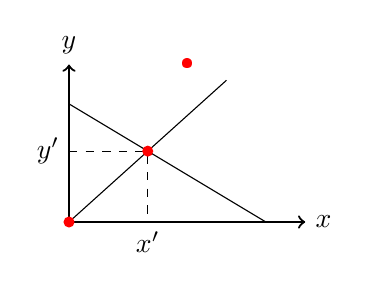
\begin{tikzpicture}
    \draw [<->,thick] (0,2) node (yaxis) [above] {$y$}
        |- (3,0) node (xaxis) [right] {$x$};
    \draw (0,0) coordinate (a_1) -- (2,1.8) coordinate (a_2);
    \draw (0,1.5) coordinate (b_1) -- (2.5,0) coordinate (b_2);
    \coordinate (c) at (intersection of a_1--a_2 and b_1--b_2);
    \draw[dashed] (yaxis |- c) node[left] {$y'$}
        -| (xaxis -| c) node[below] {$x'$};
    %
    \fill[red] (0,0) circle (2pt);
    \draw (0,0) node {\pdftooltip{\rule{0pt}{0.5cm}\rule{0.5cm}{0pt}}{Origin}};
    %
    \draw[red] (1.5,2) node {\pdftooltip{\textbullet}{1.5,2.0}};
    %
    \fill[red] (c) circle (2pt)
    let
        \p1 = (current path bounding box.south west),
        \p2 = (current path bounding box.north east)
    in
    node at (current path bounding box)
    {\pdftooltip{\rule{\dimexpr\x2-\x1\relax}{0pt}\rule{0pt}{\dimexpr\y2-\y1\relax}}%
    {This is the intersection point\textCR of the two lines!}};   
\end{tikzpicture}
\hspace{1cm}
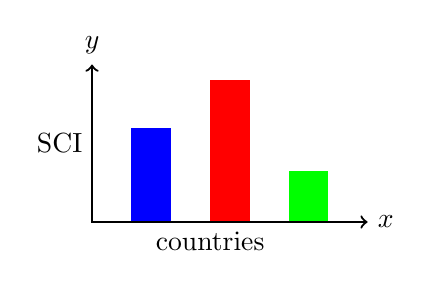
\begin{tikzpicture}
    \draw (1.5,0) node[below] {countries};
    \draw (0,1) node[left] {\pdftooltip{SCI}{Sausage Consumption Index}};
    \fill[blue] (0.5,0) rectangle (1,1.2)
    let
        \p1 = (current path bounding box.south west),
        \p2 = (current path bounding box.north east)
    in
    node at (current path bounding box)
    % these calculations are based on scale factor 1 otherwise use:
    % \dimexpr(scale factor)\dimexpr\x2-\x1\relax\relax
    {\pdftooltip{\rule{\dimexpr\x2-\x1\relax}{0pt}\rule{0pt}{\dimexpr\y2-\y1\relax}}%
    {USA: 120}};
    \fill[red] (1.5,0) rectangle (2,1.8)
    let
        \p1 = (current path bounding box.south west),
        \p2 = (current path bounding box.north east)
    in
    node at (current path bounding box)
    {\pdftooltip{\rule{\dimexpr\x2-\x1\relax}{0pt}\rule{0pt}{\dimexpr\y2-\y1\relax}}%
    {Germany: 180}};
    \fill[green] (2.5,0) rectangle (3,0.65)
    let
        \p1 = (current path bounding box.south west),
        \p2 = (current path bounding box.north east)
    in
    node at (current path bounding box)
    {\pdftooltip{\rule{\dimexpr\x2-\x1\relax}{0pt}\rule{0pt}{\dimexpr\y2-\y1\relax}}%
    {South Africa: 65}};
    \draw [<->,thick] (0,2) node (yaxis) [above] {$y$}
        |- (3.5,0) node (xaxis) [right] {$x$};
\end{tikzpicture}

\bigskip\bigskip
You can use tooltips with simple \pdftooltip{\textcolor{red}{words}}{This is a tooltip!} or chemical notation like: $\pdftooltip{H_{2}SO_{4}}{Sulfuric acid}$ 

\bigskip\bigskip
It also works in equations: \[\pdftooltip[mathstyle=\displaystyle]{\sum_{i=1}^{n}i=\frac{1}{2}n\cdot(n+1)}{little Gau�}\]
\end{document} 